\documentclass{rptuma}

% personal includings
\usepackage{lipsum}  

% thesis variables
\newdate{thesisDate}{13}{10}{2000}
\subject{Master Thesis}
\title{Title}
\author{Author's Name}
%\authoremail{Email@rptu.de}  %(optional, include rptuma.cls line 197)
%\authorid{123456}  %(optional, include rptuma.cls line 199)
\department{University of Kaiserslautern-Landau\\Department of Computer Science\\Distributed Systems Lab}
\supervisortitle{Examiner:}
%\secondsupervisortitle{}
\supervisor{Prof. Dr.-Ing. Jens B. Schmitt}
\secondsupervisor{M. Sc. Supervisor Name}
% If you want to add a dedication, please uncomment the following line
%\dedication{Add here a dedication}

\begin{document}

\maketitle

\makedeclaration

% Uncomment the next line to add a dedication
%\makededication


\pagenumbering{roman}
\setcounter{page}{1}

\chapter*{Abstract}
English

\chapter*{Zusammenfassung}	
Deutsche

\tableofcontents

\listoffigures

\listoftables

\cleardoublepage

\pagenumbering{arabic}

\chapter{Introduction}
\label{chap:intro}

% useful options for the figure- & table-environments: \begin{figure}[htbp]
\begin{figure}
	\centering
	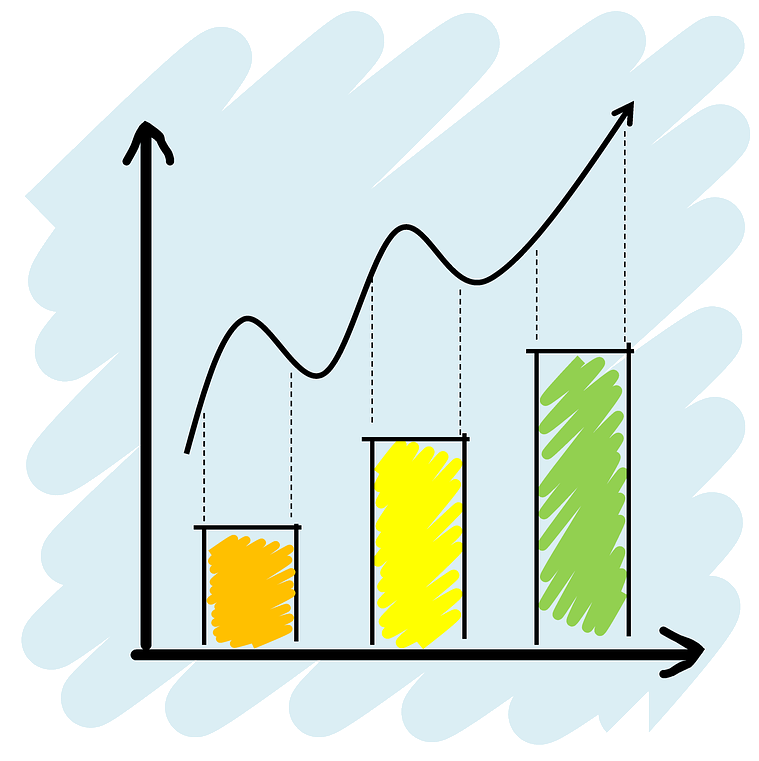
\includegraphics[width=.3\textwidth]{img/generic_graph.png}
	\caption{A very important graph.}
	\label{fig:intro.importantGraph}
\end{figure}

According to Alice et. al. \cite{alice2024paper} the data in Figure \ref{fig:intro.importantGraph} displays some very important properties, which will be explained in more detail in Chapter \ref{chap:related}. It is important to always reference a figure in the text.

When citing a website that is not a persistent document as a paper, it is required to archive the website to make it transparent, which information was available at that time. Therefore one may recall the website of our group \cite{disco2021website} in the specified way.

\lipsum[1]

\chapter{Related Work}
\label{chap:related}
\lipsum[3]

\begin{table}
\centering
\begin{tabular}{|c|r|l|}
\hline
Type & Data 1 & Data 2\\
\hline
\hline
a & 100 & 130\\
\hline
b & 104 & 115\\
\hline
c & 103 & 123\\
\hline
\end{tabular}
\caption{Example Table.}
\label{tab:related.table}
\end{table}

\lipsum[4]

\chapter{Another chapter}
\label{chap:another}
\lipsum[5]

\section{With}
\label{sec:anotehr.with}
\lipsum[6]

\section{Sections}
\label{sec:another.section}
\lipsum[7]

\subsection{And}
\label{subsec:another.section.and}
\lipsum[8]

\subsection{Subsections}
\label{subsec:another.section.subsection}
\lipsum[9]

\bibliographystyle{ieeetr}
\bibliography{literature}
\end{document}
